\begin{frame}{Circuito de interconexión}
	\begin{itemize}
		\only<1>{
			\item Versión 1\\
			\centering
			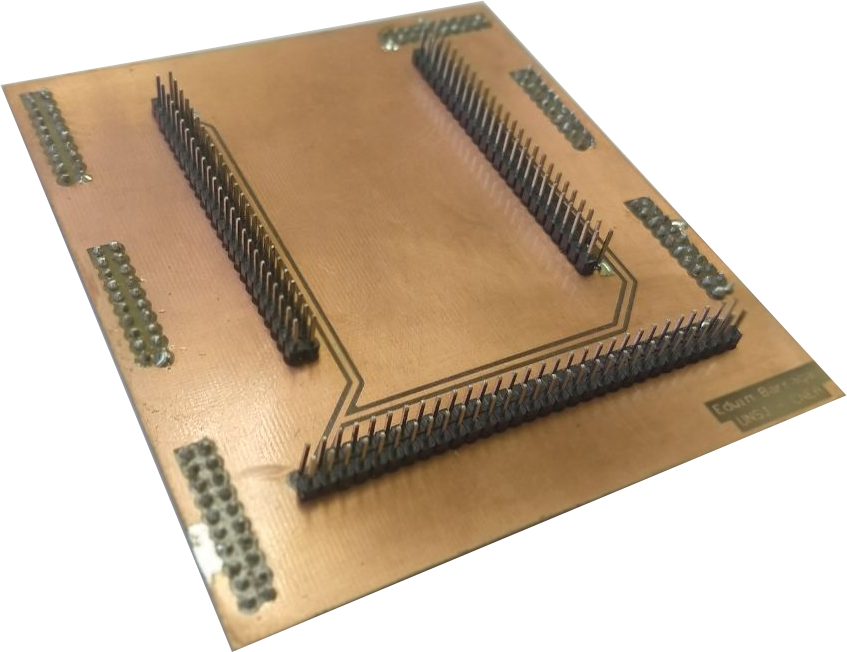
\includegraphics[width=.45\textwidth]{61v1anverso}
			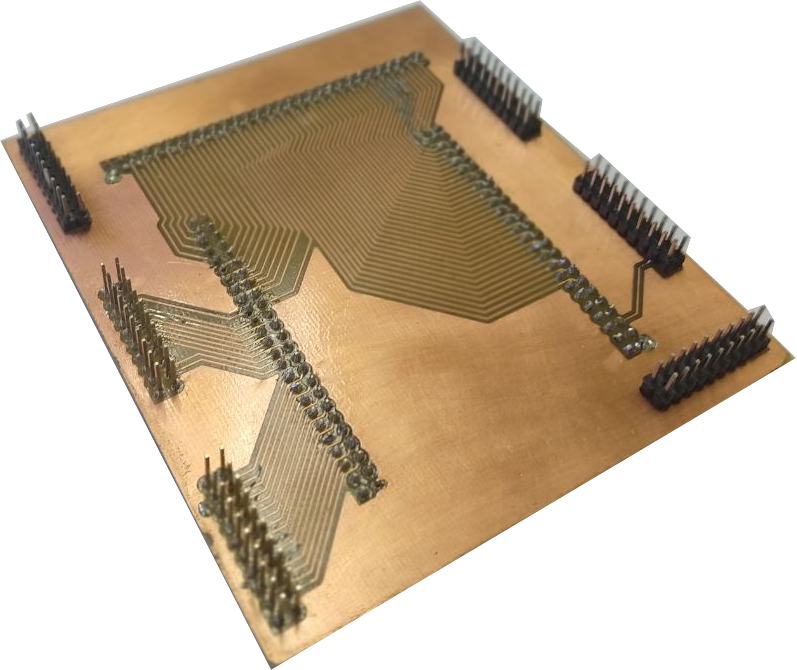
\includegraphics[width=.45\textwidth]{62v1reverso}
		}			
		\only<2>{
			\item Versión 2\\
			\centering
			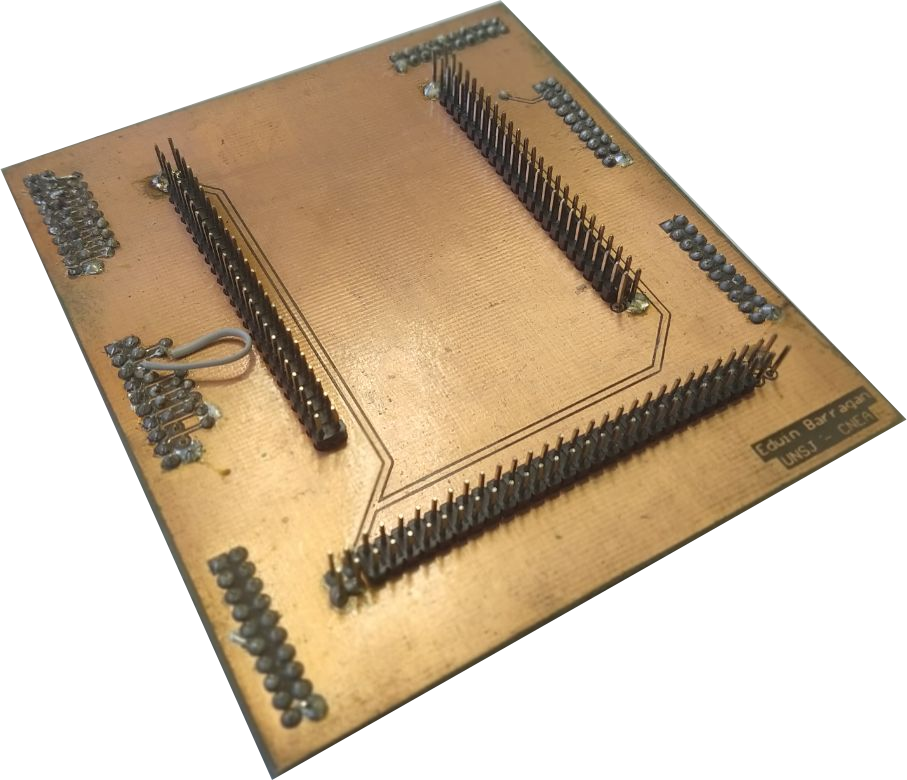
\includegraphics[width=.45\textwidth]{63v2anverso}
			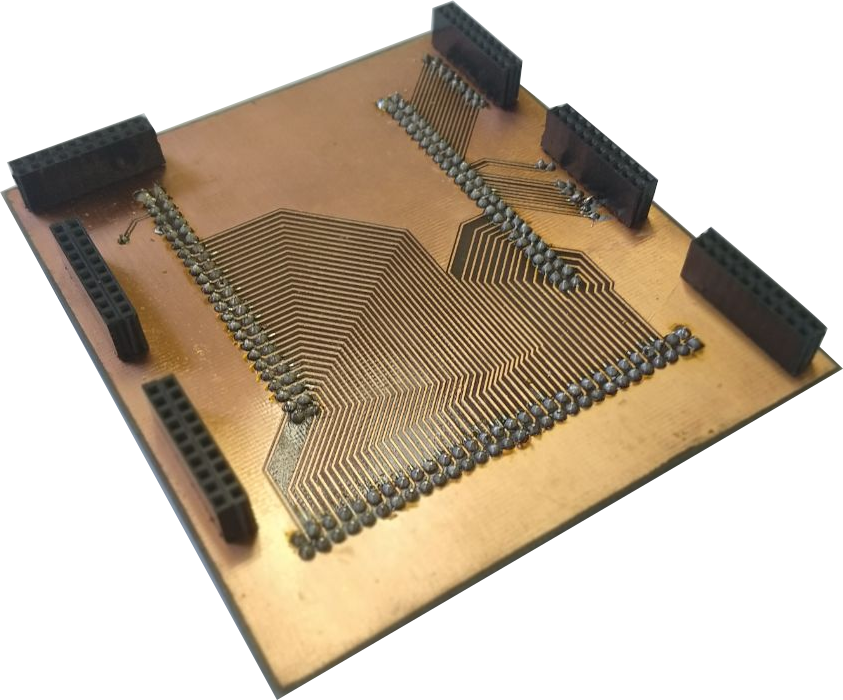
\includegraphics[width=.45\textwidth]{64v2reverso}
		}
		\only<3>{
			\item Versión 3\\
			\centering
			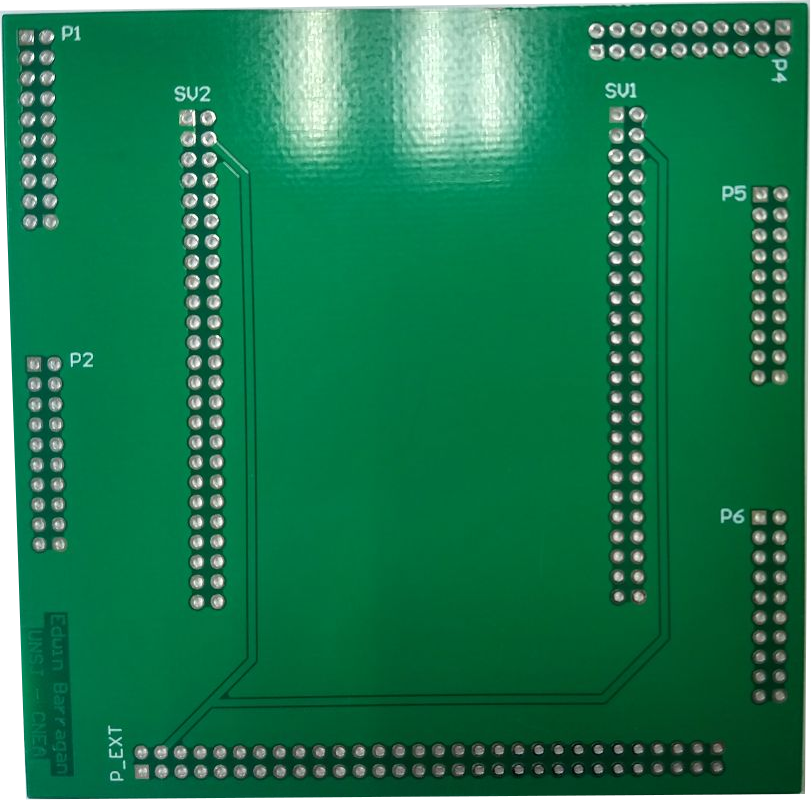
\includegraphics[width=.45\textwidth]{65v3anverso}
			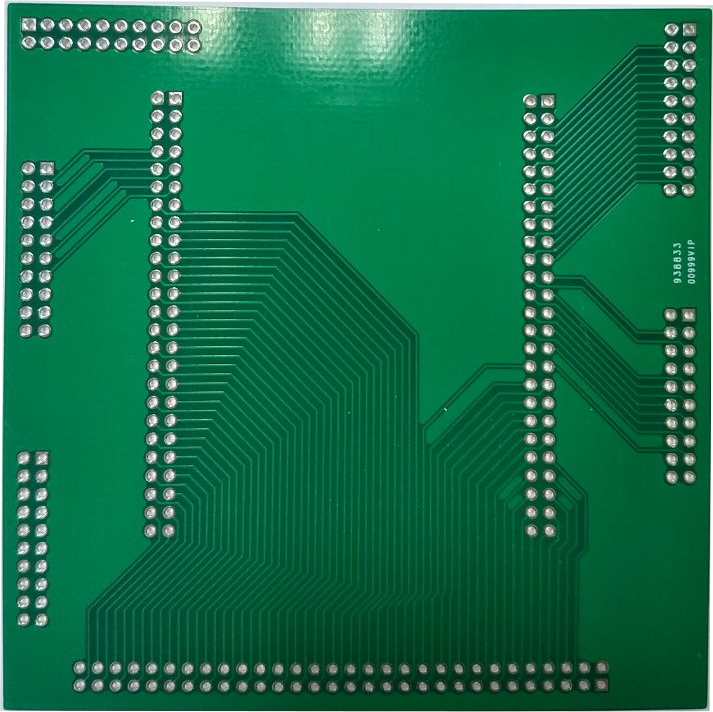
\includegraphics[width=.45\textwidth]{66v3reverso}
		}
	\end{itemize}
\end{frame}
\begin{frame}{Sistema completo}
	\centering
	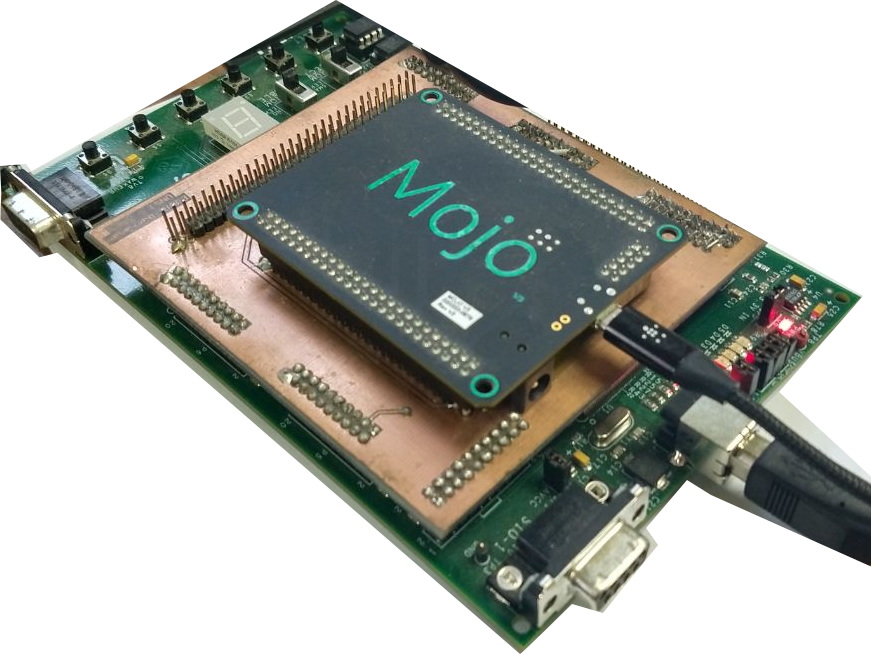
\includegraphics[width=.6\textwidth]{fisico}
\end{frame}
